\documentclass[12pt]{article}\usepackage[]{graphicx}\usepackage[]{color}
%% maxwidth is the original width if it is less than linewidth
%% otherwise use linewidth (to make sure the graphics do not exceed the margin)
\makeatletter
\def\maxwidth{ %
  \ifdim\Gin@nat@width>\linewidth
    \linewidth
  \else
    \Gin@nat@width
  \fi
}
\makeatother

\definecolor{fgcolor}{rgb}{0.345, 0.345, 0.345}
\newcommand{\hlnum}[1]{\textcolor[rgb]{0.686,0.059,0.569}{#1}}%
\newcommand{\hlstr}[1]{\textcolor[rgb]{0.192,0.494,0.8}{#1}}%
\newcommand{\hlcom}[1]{\textcolor[rgb]{0.678,0.584,0.686}{\textit{#1}}}%
\newcommand{\hlopt}[1]{\textcolor[rgb]{0,0,0}{#1}}%
\newcommand{\hlstd}[1]{\textcolor[rgb]{0.345,0.345,0.345}{#1}}%
\newcommand{\hlkwa}[1]{\textcolor[rgb]{0.161,0.373,0.58}{\textbf{#1}}}%
\newcommand{\hlkwb}[1]{\textcolor[rgb]{0.69,0.353,0.396}{#1}}%
\newcommand{\hlkwc}[1]{\textcolor[rgb]{0.333,0.667,0.333}{#1}}%
\newcommand{\hlkwd}[1]{\textcolor[rgb]{0.737,0.353,0.396}{\textbf{#1}}}%

\usepackage{framed}
\makeatletter
\newenvironment{kframe}{%
 \def\at@end@of@kframe{}%
 \ifinner\ifhmode%
  \def\at@end@of@kframe{\end{minipage}}%
  \begin{minipage}{\columnwidth}%
 \fi\fi%
 \def\FrameCommand##1{\hskip\@totalleftmargin \hskip-\fboxsep
 \colorbox{shadecolor}{##1}\hskip-\fboxsep
     % There is no \\@totalrightmargin, so:
     \hskip-\linewidth \hskip-\@totalleftmargin \hskip\columnwidth}%
 \MakeFramed {\advance\hsize-\width
   \@totalleftmargin\z@ \linewidth\hsize
   \@setminipage}}%
 {\par\unskip\endMakeFramed%
 \at@end@of@kframe}
\makeatother

\definecolor{shadecolor}{rgb}{.97, .97, .97}
\definecolor{messagecolor}{rgb}{0, 0, 0}
\definecolor{warningcolor}{rgb}{1, 0, 1}
\definecolor{errorcolor}{rgb}{1, 0, 0}
\newenvironment{knitrout}{}{} % an empty environment to be redefined in TeX

\usepackage{alltt}
\usepackage[osf]{garamondx}
\usepackage[garamondx,cmbraces]{newtxmath}
\usepackage{marginnote}
\usepackage[top=2cm, bottom=2cm, outer=3cm, inner=3cm, heightrounded, 
            marginparwidth=2cm, marginparsep=0.5cm]{geometry}
\usepackage{setspace}
\usepackage[backend=biber, style=authoryear, uniquelist=minyear, uniquename=false]{biblatex}
\usepackage[acronym,nonumberlist]{glossaries}
\usepackage{multirow}
\usepackage{cleveref}
\usepackage{array}

\newcommand{\defn}[1]{\textit{#1}}
\newcommand{\software}[1]{\textit{#1}}

\newcommand{\set}[1]{\left\lbrace#1\right\rbrace}
\newcommand{\sett}[1]{\{#1\}}
\renewcommand{\emptyset}{\varnothing}
\renewcommand{\vec}[1]{\mathbf{#1}}
\renewcommand{\star}[1]{#1^*}
\renewcommand{\d}{\mathrm{d}\,}

\DeclareMathOperator*{\argmin}{arg\,min}
\DeclareMathOperator*{\argmax}{arg\,max}

\DeclareMathOperator{\Exponential}{Exponential}
\DeclareMathOperator{\Uniform}{Uniform}
\DeclareMathOperator{\E}{E}
\DeclareMathOperator{\Var}{Var}

\DeclareMathOperator{\inc}{in}
\DeclareMathOperator{\out}{out}

\newcommand{\N}{\mathcal{N}}
\renewcommand{\L}{\mathcal{L}}

\newacronym{BA}{BA}{Barab\'asi-Albert}
\newacronym{SI}{SI}{susceptible-infected}
\newacronym{kSVM}{kSVM}{kernel support vector machine}
\newacronym{nLTT}{nLTT}{normalized lineages-through-time}
\newacronym{SMC}{SMC}{sequential Monte-Carlo}
\newacronym{ABC}{ABC}{approximate Bayesian computation}
\newacronym{MSM}{MSM}{men who have sex with men}
\newacronym{HPD}{HPD}{highest posterior density}
\newacronym{GTR}{GTR}{general time-reversible}
\newacronym{MCMC}{MCMC}{Markov chain Monte Carlo}
\newacronym{MAP}{MAP}{maximum \textit{a posteriori}}
\newacronym{IDU}{IDU}{injection drug user}

\graphicspath{{../figures/}}
\newcommand{\tablepath}{../tables}
\def\figwidth{0.8\textwidth}

\title{Phylodynamic inference of contact network parameters through approximate
Bayesian computation}
\author{Rosemary M. McCloskey \and Richard H. Liang \and Art F.Y. Poon}

\addbibresource{papers.bib}

\frenchspacing
\onehalfspacing
\IfFileExists{upquote.sty}{\usepackage{upquote}}{}
\begin{document}



\maketitle

\section*{Background}

When an infectious disease spreads through a population, transmissions are
generally more likely to occur between certain pairs of individuals. Such pairs
must have a particular mode of contact with one another, which varies with the
mode of transmission of the disease. For airborne pathogens, physical proximity
may be sufficient, but for sexually transmitted diseases, either sexual or
blood-to-blood contact is required. The set of links between individuals along
which transmission can occur is called the contact
network~\autocite{klovdahl1985social, morris1993epidemiology}. The structure of
the contact network underlying an epidemic can profoundly impact the speed and
pattern of the epidemic's expansion. Network structure can influence the
prevalence trajectory~\autocite{o2010contact} and epidemic
threshold~\autocite{barthelemy2005dynamical}, in turn affecting the estimates
of quantities such as effective population
size~\autocite{goodreau2006assessing}. From a public health perspective,
contact networks have been explored as tools for curtailing epidemic spread, by
way of interventions targeted to well-connected
nodes~\autocite{wang2015targeting}. True contact networks are a challenging
type of data to collect, requiring extensive epidemiological
investigation~\autocite{welch2011statistical}.

Viral sequence data, on the other hand, has become relatively inexpensive and
straightforward to collect on a population level. Due to the high mutation rate
of RNA viruses, epidemiological processes impact the course of viral evolution,
thereby shaping the intra-host viral
phylogeny~\autocite{drummond2003measurably}. The term ``phylodynamics'' was
coined to describe this interaction, as well as the growing family of inference
methods to estimate epidemiological parameters from viral
phylogenies~\autocite{grenfell2004unifying}. These methods have revealed
diverse properties of local viral outbreaks, from basic reproductive
number~\autocite{stadler2011estimating}, to the degree of
clustering~\autocite{hughes2009molecular}, to the elevated transmission risk
during acute infection~\autocite{volz2012simple}. On the other hand, although
sophisticated methods have been developed for fitting complex population
genetic models to phylogenies~\autocite{rasmussen2014phylodynamic}, inference
of structural network parameters has to date been limited. However, it has been
shown that network structure has a tangible impact on phylogeny
shape~\autocite{leventhal2012inferring, colijn2014phylogenetic,
goodreau2006assessing, robinson2013dynamics}, suggesting that such statistical
inference might be possible~\autocite{welch2011statistical}.

Survey-based studies of sexual networks~\autocite{liljeros2001web,
schneeberger2004scale} have found that sexual contact networks are best
described by a preferential attachment model \autocite[although there has been
some disagreement, see][]{jones2003assessment}. Under these models, nodes with
a high number of contacts attract new connections at an elevated rate. Networks
produced by preferential attachment have a power-law degree distribution,
meaning that the number of nodes of degree $k$ is proportional to $k^\gamma$
for some constant $\gamma$. These networks are also referred to as
``scale-free''. The first contact network model incorporating preferential
attachment was introduced by \textcite{barabasi1999emergence}, and is now
referred to as the \gls{BA} model. Under this model, networks are formed by
iteratively adding nodes with $m$ new edges each. These new edges are joined to
existing nodes of degree $k$ with probability proportional to $k^\alpha$, so
that nodes of high degree tend to attract more connections (in the original
paper, only $\alpha = 1$ was investigated).

Previous work offers precedent for the possibility of statistical inference of
structural network parameters. \textcite{britton2002bayesian} develop a
Bayesian approach to estimate the edge density in an Erd\H{o}s-R\'enyi
network~\autocite{erdos1960evolution} given observed infection dates, and
optionally recovery dates. Their approach was later extended by
\textcite{groendyke2011bayesian} and applied to a much larger data set of 188
individuals. \textcite{brown2011transmission} analysed the degree distribution
of an approximate transmission network, estimated based on genetic similarity
and estimated times of infection, relating 60\% of HIV infected \gls{MSM} in
the United Kingdom. The transmission network is a subgraph of the contact
network which includes only those edges which have already led to a new
infection. The authors found that a Waring distribution, which is produced by a
different preferential attachment model, was a good fit to their estimated
network.

Standard methods of model fitting involve calculation of the likelihood of
observed data under the model. In maximum likelihood estimation, a quantity
proportional to the likelihood is optimized, often through a standard
multi-dimensional numerical optimization procedure. Bayesian methods integrate
prior information by optimizing the posterior probability instead. To avoid
calculation of a normalizing constant, Bayesian inference is often performed
using \gls{MCMC}. Rather than calculating explicit likeilihoods, \gls{MCMC}
uses likelihood \emph{ratios} in which the normalizing constant cancel out.
Unfortunately, it is generally difficult to explicitly calculate the likelihood
of an observed transmission tree under a contact network model, even up to a
normalizing constant. To do so, it would be necessary to integrate over all
possible networks, and also over all possible labellings of the internal nodes
of the transmission tree. While it is not known (to us) whether such
integration is tractable, a simpler alternative is offered by likelihood-free
methods, namely \gls{ABC}. \gls{ABC} leverages the fact that, although
calculating the likelihood may be impossible, generating simulated datasets
according to a model is often straightforward. If our model fits the data well,
the simulated data it produces should be similar to the observed data. More
formally, if $D$ is the observed data, the posterior distribution $f(\theta
\mid D)$ on model parameters $\theta$ is replaced as the target of statistical
inference by $f(\theta \mid \rho(\hat{D}, D) < \varepsilon)$, where $\rho$ is a
distance function, $\hat{D}$ is a simulated dataset according to $\theta$, and
$\varepsilon$ is a small tolerance~\autocite{sunnaker2013approximate}. In the
specific case when $\rho$ is a kernel function, the approach is known as
kernel-\gls{ABC}~\autocite{nakagome2013kernel, poon2015phylodynamic}.

Here, we apply kernel-\gls{ABC} to the problem of statistical inference of
contact network parameters from an estimated transmission tree, using the tree
kernel developed by \textcite{poon2013mapping}. We then estimate the parameters
of the \gls{BA} model on a variety of simulated and real data sets. Our results
show that the attachment power parameter $\alpha$ can be inferred with
reasonable accuracy, and can vary considerably between epidemics from different
settings.

\section*{Methods}

We implemented a Gillespie simulation algorithm~\autocite{gillespie1976general}
for simulating epidemics and transmission trees over static contact networks,
in the same fashion as several previous studies
\autocite[\textit{e.g.}][]{o2010contact, robinson2013dynamics,
leventhal2012inferring, groendyke2011bayesian, goodreau2006assessing}. To check
that our implementation was correct, we reproduced Figure 1A of
\textcite{leventhal2012inferring} (our \cref{fig:sf1}), which plots the
unbalancedness of transmission trees simulated over four network models at
various levels of pathogen transmissibility. Our program is freely available at
\url{https://github.com/rmcclosk/netabc}.

We chose to study the \gls{BA} network model~\autocite{barabasi1999emergence}.
In addition to $m$ and $\alpha$, we investigated the parameters $N$, which
denotes the total number of nodes in the network, and $I$, which is the number
of infected nodes at which to stop the simulation and sample the transmission
tree. Nodes in our networks followed simple \gls{SI} dynamics, meaning that
they became infected at a rate proportional to their numbers of infected
neighbours, and never recovered. For all analyses, the transmission trees'
branch lengths were scaled by dividing by their mean. We used the 
\software{igraph} library's implementation of the \gls{BA}
model~\autocite{csardi2006igraph} to generate the graphs. The analyses were run
on Westgrid (\url{https://www.westgrid.ca/}) and a local computer cluster.

\subsection*{Kernel classifiers}

We used the phylogenetic kernel developed by \textcite{poon2013mapping} to test
whether the parameters of the \gls{BA} model had an effect on tree shape. We
simulated 100 networks under each of three different values of $\alpha$: 0.5,
1.0, and 1.5 (300 networks total). The other parameters were fixed to the
following values: $N$ = 5000, $I$ = 1000, and $m$ = 2. A transmission tree with
500 tips was simulated over each network (300 transmission trees total). The
300 trees were compared pairwise with the tree kernel to form a $300 \times
300$ kernel matrix. The kernel meta-parameters $\lambda$ (the ``decay
factor''), and $\sigma$ (the ``radial basis function
variance'')~\autocite[see][]{poon2013mapping}, were set to 0.3 and 4
respectively. We constructed a \gls{kSVM} classifier for $\alpha$ using the
\software{kernlab} package~\autocite{karatzoglou2004kernlab}, and evaluated its
accuracy with 1000 two-fold cross-validations.

Three similar experiments were performed for the other \gls{BA} model
parameters (one experiment per parameter). $m$ was varied between 2, 3, and 4;
$I$ between 500, 1000, and 2000; and $N$ between 3000, 5000, and 8000. The
parameters not being tested were fixed at the values $N$ = 5000, $I$ = 1000,
$m$ = 2, and $\alpha$ = 1. Thus, we performed a total of four kSVM
cross-validations, one for each of the \gls{BA} model parameters $\alpha$, $I$,
$m$, and $N$.

We repeated these four cross-validations with different values of $\lambda$
(0.2, 0.3, and 0.4) and $\sigma$ ($2^{-3}$, $2^{-2}$, \ldots, $2^3$), as well
as on trees with differing numbers of tips (100, 500, and 1000) and in
epidemics of differing size $I$ (500, 1000, and 2000). When evaluating the
classifier for $I$, we did not consider trees with 1000 tips, because one of
the tested $I$ values was 500, and the number of tips cannot be larger than
$I$.

For each of the four parameters, we also tested univariate classifier based on
Sackin's index~\autocite{shao1990tree} and an ordinary SVM based on the
\gls{nLTT} statistic~\autocite{janzen2015approximate}.

\subsection*{ABC simulations}

We implemented the adaptive \gls{SMC} algorithm for \gls{ABC} developed by
\textcite{del2012adaptive}. To check that our implementation was correct, we
applied it to the same mixture of Gaussians used by
\citeauthor{del2012adaptive} to demonstrate their method (originally used
by~\textcite{sisson2007sequential}). We were able to obtain a close
approximation to the function (see \cref{fig:smctest}), and attained the
stopping condition used by the authors in a comparable number of steps.

We simulated three transmission trees, each with 500 tips, under every element
of the Cartesian product of these parameter values: $N$ = 5000, $I$ =
\sett{1000, 2000}, $m$ = \sett{2, 3, 4}, and $\alpha$ = \sett{0.0, 0.5, 1,
1.5}. This produced a total of 24 parameter combinations $\times$ three trees
per combination = 72 trees total. The adaptive \gls{ABC} algorithm was applied
to each tree with these priors: $m \sim$ Uniform(1, 5), $\alpha \sim$
Uniform(0, 2), and $(N, I)$ jointly uniform on the triangular region \{$500
\leq N \leq 15000$, $500 \leq I \leq 5000$, $I \leq N$\}. Following
\textcite{del2012adaptive} and \textcite{beaumont2009adaptive}, all proposals
were Gaussian, with variance equal to twice the empirical variance of the
particles. The algorithm was run with 1000 particles, 5 simulated datasets per
particle, and the ``quality'' parameter controlling the decay rate of the
tolerance $\varepsilon$ set to 0.95. We used the same stopping criterion as
\citeauthor{del2012adaptive}, namely when the \gls{MCMC} acceptance rate
dropped below 1.5\%. Point estimates for the parameters were obtained by taking
the highest point of an estimated kernel density on the final set of particles,
using the \software{density} function with the default parameters in
\software{R}. \gls{HPD} intervals were calculated with the
\software{HPDinterval} function from the \software{R} package
\software{coda}~\autocite{plummer2006coda}.

Two further analyses were performed to address potential sources of error. To
evaluate the effect of model misspecification in the case of heterogeneity
among nodes, we generated a network where half the nodes were attached with
power $\alpha$ = 0.5, and the other half with power $\alpha$ = 1.5. The other
parameters for this network were $N$ = 5000, $I$ = 1000, and $m$ = 2. To
investigate the effects of potential sampling bias, we simulated a transmission
tree where the tips were sampled in a peer-driven fashion, rather than at
random. That is, the probability to sample a node was twice as high if any of
that node's network peers had already been sampled. The parameters of this
network were $N$ = 5000, $I$ = 2000, $m$ = 2, and $\alpha$ = 0.5.

\subsection*{Investigation of published data}

We applied our kernel-ABC method to several published HIV datasets. Because the
\gls{BA} model generates networks with a single connected component, we
specifically searched for datasets which originated from existing clusters,
either phylogenetically or geographically defined. Characteristics of the
datasets we investigated are given in \cref{tab:data}.

\begin{table}[ht]
  \centering
  \begin{tabular}{ccccc}
  Reference & Sequences ($n$) & Location & Risk group & Gene \\
  \hline
  \textcite{wang2015targeting} & 173 & Beijing, China & MSM & \textit{pol} \\
  \textcite{cuevas2009hiv} & 287 & Basque Country, Spain & mixed & \textit{pol} \\
  \textcite{novitsky2013phylogenetic} & \multirow{2}{*}{180} &
  \multirow{2}{*}{Mochudi, Botswana} & \multirow{2}{*}{HET} &
  \multirow{2}{*}{\textit{env}} \\ \textcite{novitsky2014impact} \\
  \textcite{li2015hiv} & 280 & Shanghai, China & MSM & \textit{pol} \\
  \textcite{niculescu2015recent} & 136 & Romania & IDU & \textit{pol} \\
  \hline
\end{tabular}

  \caption{Characteristics of published datasets investigated with kernel-ABC.
  Acronyms: MSM, men who have sex with men; IDU, injection drug users.}
  \label{tab:data}
\end{table}

We downloaded all sequences associated with each study from GenBank. For the
\textcite{novitsky2014impact} data, each sequence was aligned pairwise to the
HXB2 reference sequence (Genbank accession number HIVHXB2CG) and the
hypervariable regions were clipped out with BioPython version
1.66+~\autocite{cock2009biopython}. Sequences were multiply aligned using
\software{MUSCLE} version 3.8.31 \autocite{edgar2004muscle}, and alignments
were manually inspected with \software{Seaview} version 4.4.2
\autocite{gouy2010seaview}. Phylogenies were constructed from the nucleotide
alignments by approximate maximum likelihood using \software{FastTree2} version
2.1.7 with the \gls{GTR} model. Transmission trees were estimated by rooting
and time-scaling the phylogenies by root-to-tip regression, using a modified
version of Path-O-Gen (distributed as part of
BEAST~\autocite{drummond2007beast}) as described
previously~\autocite{poon2015phylodynamic}. 

Two of the datasets \autocite{li2015hiv,novitsky2014impact} were initially much
larger than the others, containing 1265 and 1299 sequences respectively. To
ensure that the analyses were comparable, we reduced these to a number of
sequences similar to the smaller datasets. For the \textcite{li2015hiv} data,
we detected a cluster of size 280 using a patristic distance cutoff of 0.02 as
described previously~\autocite{poon2014impact}. Only sequences within this
cluster were carried forward. For the \textcite{novitsky2014impact} data, no
large clusters were detected using the same cutoff, so we analysed a subtree of
size 180 chosen arbitrarily.

\section*{Results}

\subsection*{Kernel classifiers}



Accuracy of the \gls{kSVM} classifiers varied based on the parameter being
tested~\cref{fig:rsquared}. Classifiers based on two other tree statistics, the
\gls{nLTT} and Sackin's index, generally exhibited worse performance than the
tree kernel, although the magnitude of the disparity varied between the
parameters. \Cref{fig:rsquared} shows the cross-validation accuracy with
$\lambda$ = 0.3, $\sigma$ = 4, $I$ = 1000, and trees of size 500. The results
were largely robust to variations in $\lambda$ and $\sigma$, although accuracy
varied between different epidemic and sampling scenarios
(\cref{fig:alphacrossv,fig:mcrossv,fig:Icrossv,fig:Ncrossv}).

The kSVM classifier for $\alpha$ had an average $R^2$ of
    0.92 
(\cref{fig:alphacrossv}). The $R^2$ of the for the SVM classifer for $\alpha$
using the \gls{nLTT} varied between
0.49
and
  0.61.
The $R^2$ of the linear regression against Sackin's index varied between
  0.73
and
  0.76.
The $I$ parameter was also classified accurately by the tree kernel
(\cref{fig:Icrossv}), with an average
$R^2$ of 
  0.93 
for 500-tip trees or 
  0.7 
for 100-tip trees. The \gls{nLTT} performed almost as well on this parameter as
the tree kernel, with $R^2$ values of
  0.83
for 500-tip trees or
  0.55
for 100-tip trees. Sackin's index was an extremely poor classifier for this
parameter, with both $R^2$ values below
  0.08.

The $m$ parameter was much harder to classify (\cref{fig:mcrossv}), with $R^2$
for the kSVM varying between 
  0.004
and
  0.36
depending on $I$ and the tree size. The \gls{nLTT} was also universally poor,
with $R^2$ below
  0.02
for all scenarios. Sackin's index fared slightly better than the \gls{nLTT},
especially on trees with a higher number of tips, with $R^2$ between
  0
and
  0.18.
Finally, the accuracy of the kSVM classifier for $N$ varied widely
(\cref{fig:Ncrossv}), from 
  0.08
to
  0.82.
The \gls{nLTT} performed well in classifying $N$ when the epidemic was large,
improving upon the tree kernel in the scenarios with $I$ = 2000 and 100- or
500-tip transmission trees ($R^2$ = 
  0.31
and
  0.53),
although it performed poorly when $I$ was 500 or 1000 (average $R^2$ =
  0.07).
Sackin's index could not classify $N$, with all $R^2$ below
  0.11.
Based on inspection of the cross-validation results, we chose to use the
meta-parameters $\lambda = 0.3$ and $\sigma = 4$ in further analyses, and not
to use Sackin's index or the \gls{nLTT}. 

\begin{figure}[ht]
  \centering
  \includegraphics[width=\textwidth]{kernel-rsquared.pdf}
  \caption{
      Cross-validation accuracy of kernel-SVM classifier (left), SVM classifier
      using \gls{nLTT} (centre), and linear regression using Sackin's index
      (right) for \gls{BA} model parameters. Kernel meta-parameters were set to
      $\lambda = 0.3$ and $\sigma = 4$. Each point was calculated based on 300
      simulated transmission trees over networks with three different values of
      the parameter being tested. Vertical lines are empirical 95\% confidence
      intervals based on 1000 2-fold cross-validations.
  }
  \label{fig:rsquared}
\end{figure}

\subsection*{ABC simulations}



Of the four parameters, $\alpha$ was the most accurately estimated, with a
median [IQR] absolute error of 
    0.11 
    [0.05-0.18].
\Cref{fig:abcpt} shows point estimates for all simulations with $m = 2$. The
results $m = 3$ and $m = 4$ were similar (\cref{fig:abcptm3,fig:abcptm4}).
Average boundaries of 95\% \gls{HPD} intervals are given in \cref{tab:abchpd}.
The accuracy of the estimates was not significantly different between values of
$m$ or $I$ (both one-way ANOVA,
    $p$ = 0.1
and 
    0.25),
although the errors when the true value of $\alpha$ was zero were
significantly greater than the other values 
    (Wilcoxon rank-sum test, $p$ = \ensuremath{6.41\times 10^{-4}}).
The error in the estimated value of $I$ was
    305.66 
    [107.76-606.59].
Errors were significantly higher for $\alpha \geq 1$
    (Wilcoxon rank-sum test, $p$ = \ensuremath{6.12\times 10^{-4}})
and for $I$ = 2000
    ($p$ = \ensuremath{1.58\times 10^{-6}}),
but not for any values of $m$
    (one-way ANOVA, $p$ = 0.33).
The $m$ parameter was estimated correctly in
    37 \%
of simulations, with an error of one in
    40 \%
and of two or more in 
    22 \%
(the only possible $m$ values were 1, 2, 3, 4, or 5). The true values of $m$
and $I$ did not significantly affect the error
    (one-way ANOVA, $p$ = 0.5 and
                          0.68).
Finally, the total number of nodes $N$ was consistently over-estimated by about
a factor of two
    (error \ensuremath{6.59\times 10^{3}} 
    [\ensuremath{4.21\times 10^{3}}-\ensuremath{8.28\times 10^{3}}]).
No other parameters influenced the accuracy of the $N$ estimates 
    (one-way ANOVA, $p \geq$ 0.72).

\begin{figure}[ht]
  \centering
  \includegraphics[width=\textwidth]{abc-point-estimate-m2.pdf}
  \caption{
    Point estimates of \gls{BA} model parameters obtained by running kernel-ABC
    on simulated phylogenies without training, for simulations with $m = 2$.
    Dotted lines indicate true values, and limits of the $y$-axes are regions
    of uniform prior density.
  }
  \label{fig:abcpt}
\end{figure}

\begin{table}[ht]
  \centering
  % latex table generated in R 3.2.3 by xtable 1.8-2 package
% Fri Jun 17 12:51:45 2016
\begin{tabular}{lr>{\raggedleft\arraybackslash}p{2.5cm}>{\raggedleft\arraybackslash}p{2.5cm}>{\raggedleft\arraybackslash}p{2.5cm}}
  \hline
Parameter & True value & Mean point estimate & Mean HPD lower bound & Mean HPD upper bound \\ 
  \hline
$\alpha$ & 0.0 & 0.36 & 0.01 & 0.81 \\ 
   & 0.5 & 0.43 & 0.04 & 0.83 \\ 
   & 1.0 & 0.90 & 0.51 & 1.09 \\ 
   & 1.5 & 1.52 & 1.26 & 1.81 \\ 
  $I$ & 1000 & 1450 & 651 & 2592 \\ 
   & 2000 & 2622 & 1114 & 4080 \\ 
  $m$ & 2 & 2.96 & 2.00 & 5.00 \\ 
   & 3 & 3.04 & 2.04 & 4.96 \\ 
   & 4 & 3.17 & 1.88 & 5.00 \\ 
  $N$ & 5000 & 9041 & 2613 & 14659 \\ 
   \hline
\end{tabular}

  \caption{Average \gls{HPD} interval widths for \gls{ABC} model parameter
           estimates.}
  \label{tab:abchpd}
\end{table}

The dispersion of the \gls{ABC} approximation to the posterior also varied
between the parameters, with narrower \gls{HPD} intervals for those with the
most accurate point estimates (\cref{tab:abchpd}). \Cref{fig:abcex} shows the
distributions for for one simulation (equivalent plots for all the simulations
can be found in supplemental data). \Gls{HPD} intervals around $\alpha$ and $I$
were narrow relative to the region of nonzero prior density, whereas the
intervals for $m$ and $N$ were more widely dispersed.

\begin{figure}[ht]
  \centering
  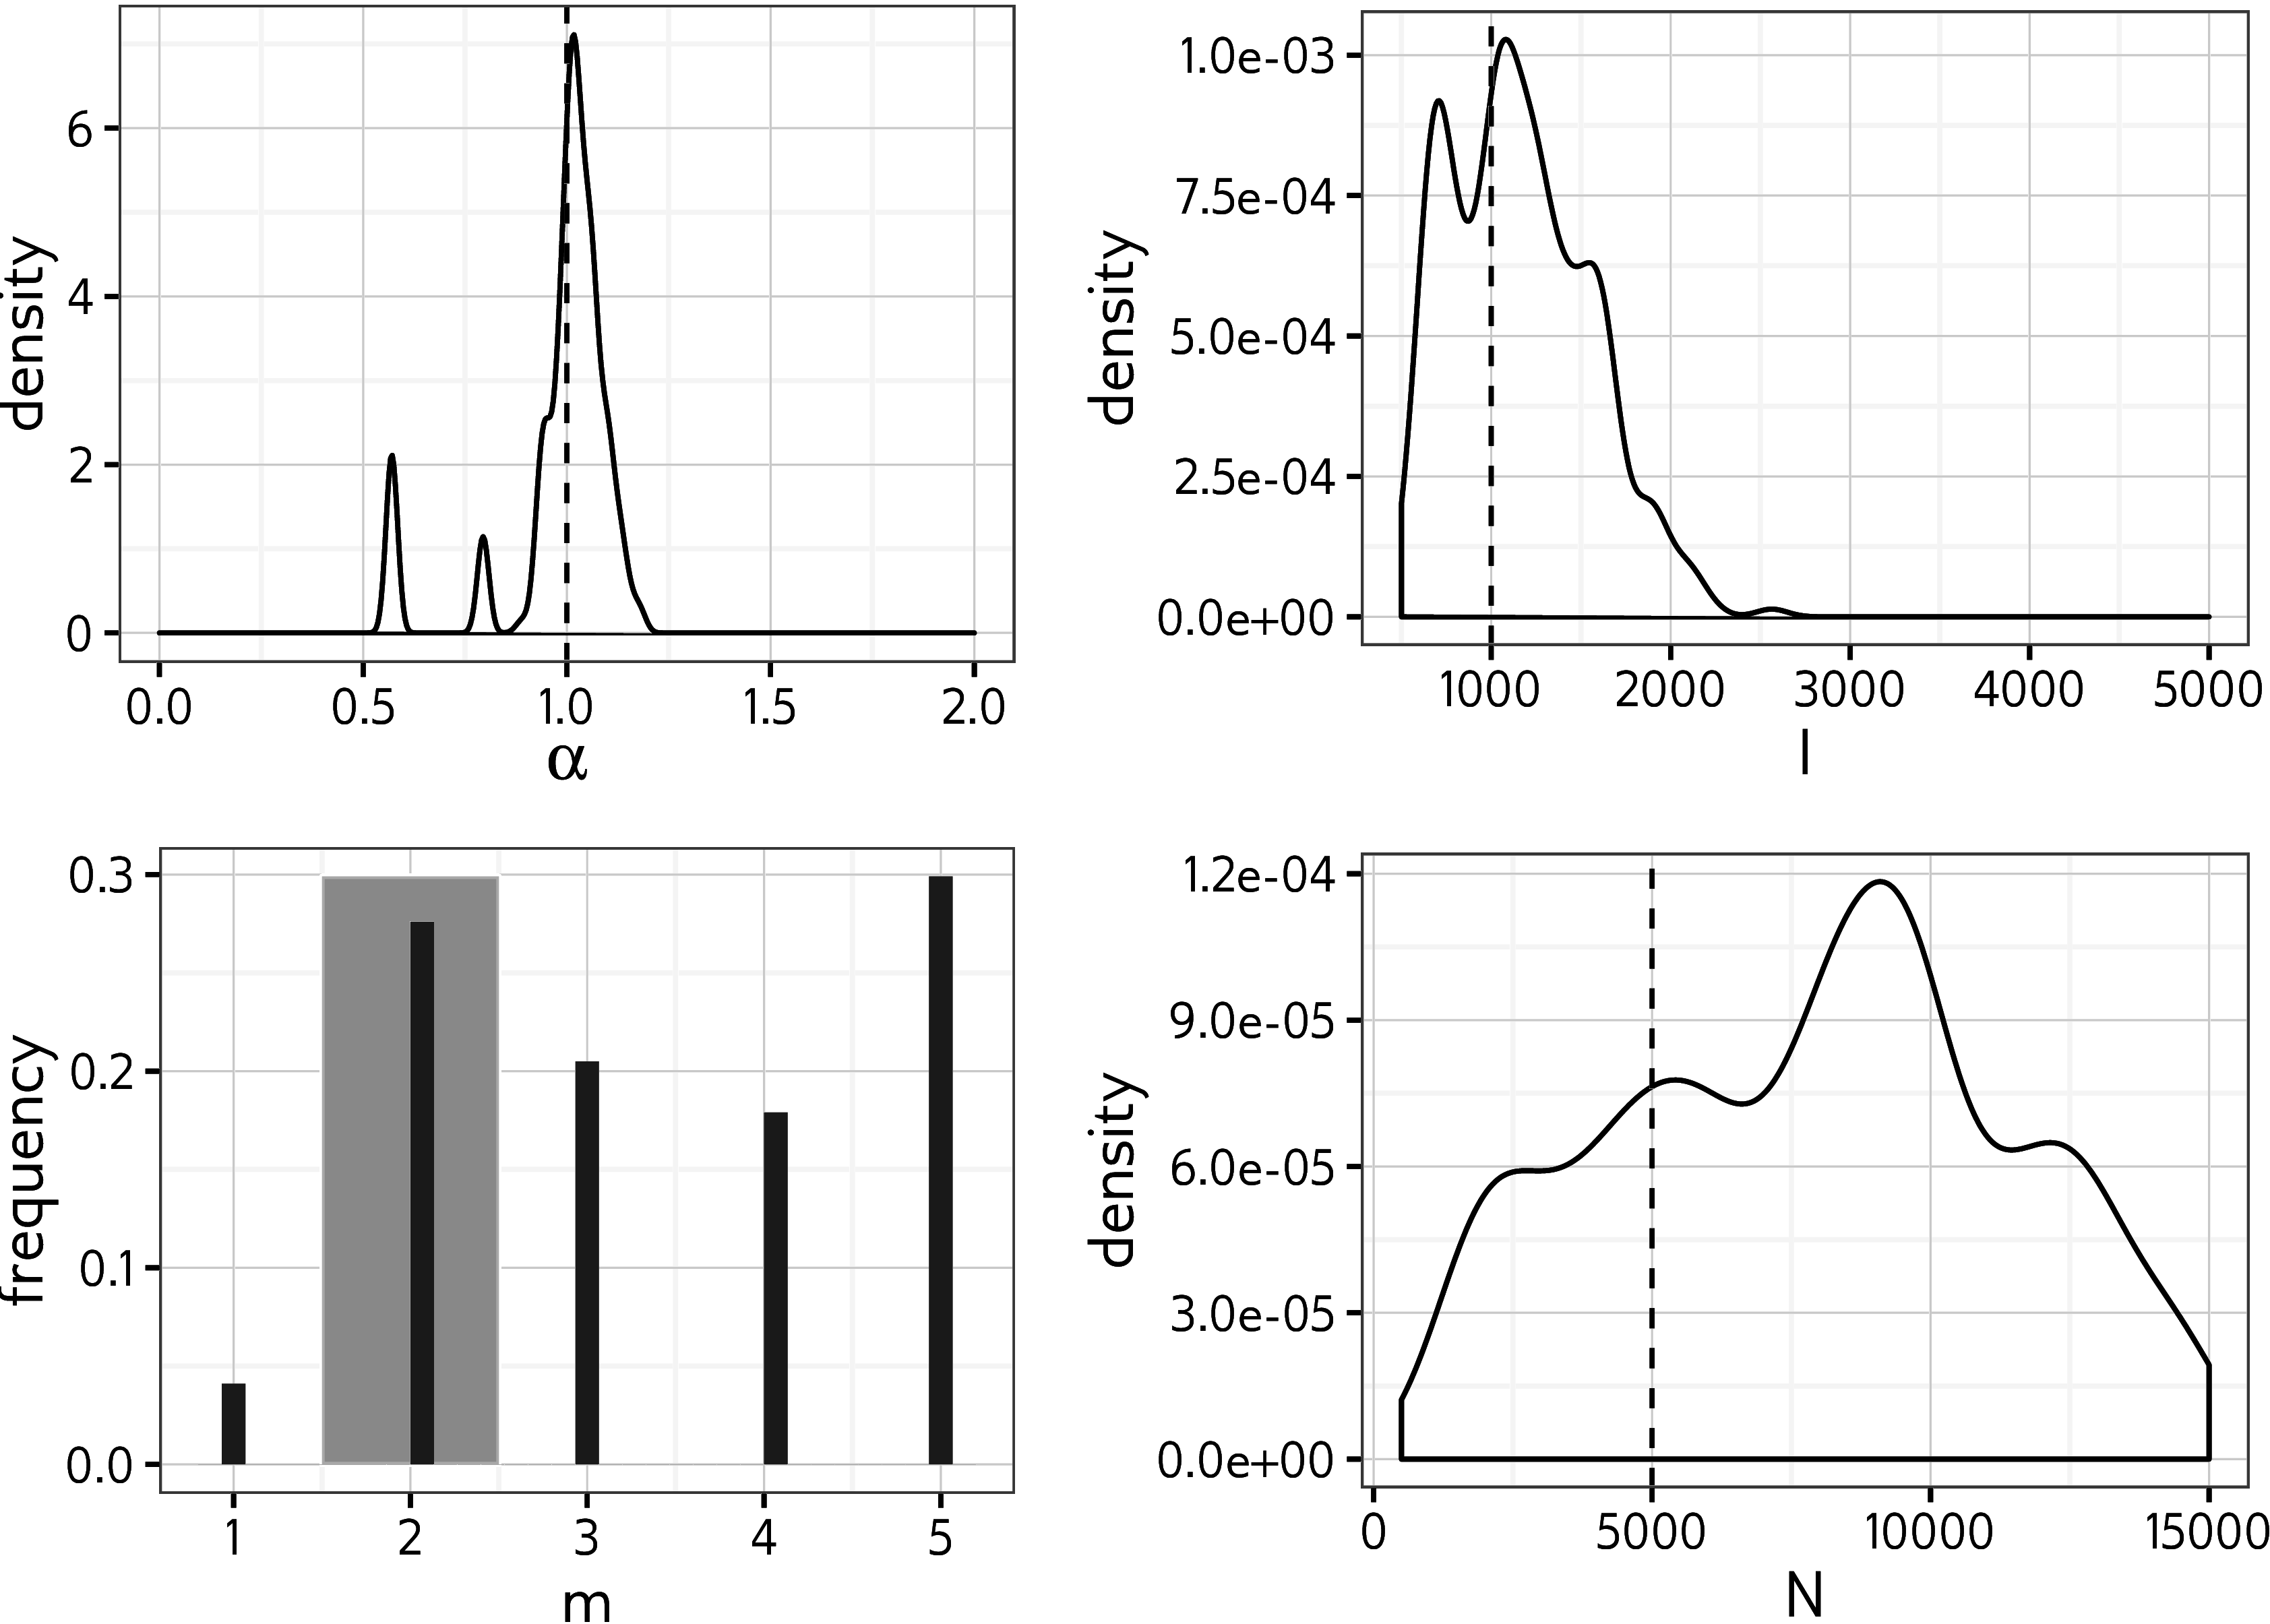
\includegraphics[width=\textwidth]{abc-posterior-example.pdf}
  \caption{Marginal estimated posterior distributions obtained with ABC on a
  single simulated dataset. Dotted lines and shaded polygon indicate true
  values.}
  \label{fig:abcex}
\end{figure}



To test the effect of model misspecification, we simulated one network where
the nodes exhibited heterogeneous preferential attachment power (half 0.5, the
other half 1.5), with $m$ = 2, $N$ = 5000, and $I$ = 1000. The \gls{MAP} [95\%
HPD] estimates for each parameter were: 
$\alpha$, 
  1 [0.75-
                           1.12];
$I$,
  5.24 [2.05-
                       5.81];
$m$,
  \ensuremath{1.04\times 10^{4}} [\ensuremath{2.27\times 10^{3}}-
                              \ensuremath{1.5\times 10^{4}}];
$N$,
  \ensuremath{1.17\times 10^{3}} [502.34-
                       \ensuremath{1.58\times 10^{3}}].



To test the effect of sampling bias, we sampled one transmission tree in a
peer-driven fashion, where the probability to sample a node was twice as high
if one of it's peers had already been sampled. The parameters for this
experiment were $N$ = 5000, $m$ = 2, $\alpha$ = 0.5, and $I$ = 2000. The
estimated values were
$\alpha$, 
  0.46 [0.03-
                           0.83];
$I$,
  3.47 [2.18-
                       5.9];
$m$,
  \ensuremath{1.08\times 10^{4}} [\ensuremath{3.11\times 10^{3}}-
                              \ensuremath{1.48\times 10^{4}}];
$N$,
  \ensuremath{2.94\times 10^{3}} [\ensuremath{1.28\times 10^{3}}-
                       \ensuremath{3.94\times 10^{3}}].

\subsection*{Real data}



There was substantial heterogeneity among the parameter estimates for the five
published HIV datasets we analysed. Two of the
datasets~\autocite{niculescu2015recent, wang2015targeting} had estimated
$\alpha$ values near unity (\gls{MAP} estimate [95\% \gls{HPD}] 
  1.06 
  [0.63-1.27]
and
  1 
  [0.41-1.16]). Another two
datasets~\autocite{li2015hiv, cuevas2009hiv} had lower estimated values and wider
\gls{HPD} intervals
  (0.77 
  [0.01-1.03]
and
  0.66 
  [0.03-0.84]). 
The \textcite{novitsky2014impact} data had an extremely low estimated $\alpha$
and a very wide \gls{HPD} interval
  0.17 
  [0.04-1.39]). 
For all the datasets except \textcite{novitsky2014impact}, estimated values of
$I$ were below 2000, with narrow \gls{HPD} intervals around two of the
datasets
  (\textcite{cuevas2009hiv}, 880.52 
  [290.7-\ensuremath{1.51\times 10^{3}}];
   \textcite{niculescu2015recent}, 175.05
  [138.74-454.51])
and wider intervals around the other two
  (\textcite{li2015hiv}, \ensuremath{1.59\times 10^{3}} 
  [284.01-\ensuremath{3.81\times 10^{3}}];
   \textcite{wang2015targeting}, 651.72
  [268.94-\ensuremath{4.24\times 10^{3}}]).
The \textcite{novitsky2014impact} data was again the outlier, with a very high
estimated $I$, and \gls{HPD} interval spanning almost the entire prior region
  (\ensuremath{7.55\times 10^{3}} 
  [228.96-\ensuremath{8.92\times 10^{3}}]).
Little information was gleaned about the $m$ parameter, with the \gls{HPD}
interval occupying the entire prior region for all datasets. The estimates of
$N$ were similarly uninformative, with the exception that the point estimate
for the \textcite{wang2015targeting} data was smaller
  (\ensuremath{5.84\times 10^{3}})
than the estimates for other datasets.

\begin{figure}[ht]
  \centering
  \includegraphics{realdata-hpd.pdf}
  \caption{
    Point estimates and 95\% \gls{HPD} intervals for \gls{BA} network
    parameters of published HIV datasets, obtained with kernel-ABC.
  }
  \label{fig:abchpd}
\end{figure}

\section*{Discussion}

Contact networks can have a strong influence on epidemic progression, and are
potentially useful as a public health tool~\autocite{wang2015targeting,
little2014using}. Despite this, few methods exist for investigating contact
network parameters in a phylodynamic framework~\autocite{groendyke2011bayesian,
brown2011transmission}. Kernel-ABC is a model-agnostic method which can be used
to investigate any quantity that affects tree shape. In this work, we developed
a kernel-ABC-based method to infer the parameters of a contact network model.
The method is general, and could be applied to any model from which contact
networks can be simulated. We demonstrated the method on the \gls{BA} model,
which is a simple model incorporating the preferential attachment feature
commonly seen in real-world networks. 

By training a kernel-SVM classifier, we found that the $\alpha$ and $I$
parameters, representing preferential attachment power and number of infected
nodes, had a strong influence on tree shape. This was reflected in the relative
accuracy of the kernel-ABC estimates of these parameters. The total number of
nodes $N$ had a weak influence on tree shape, which was most prominent when the
epidemic size $I$ and number of sampled tips were both large. The $m$
parameter, representing the number of edges created in the network per vertex,
did not produce much variation in tree shape, resulting in in both poorly
performing classifiers and uninformative kernel-ABC estimates.

$N$ was almost always significantly over-estimated using kernel-ABC. Since the
prior on $N$ and $I$ is jointly uniform on a triangular region ($I \leq N$),
there is more prior mass on high $N$ values. In retrospect, it is unreasonable
to expect good estimation of $N$, because adding more nodes to a \gls{BA}
network does not change the edge density or overall shape. This can be
illustrated by imagining that we add a small number of nodes to a network after
the epidemic simulation has already been completed. It is possible that none of
these new nodes attains a connection to any infected node. Thus, running the
simulation again on the new, larger network could produce the exact same
transmission tree as before. 

As noted by \textcite{lintusaari2016identifiability}, uniform priors on model
parameters may translate to highly informative priors on quantities of
interest. We observed an exponential relationship between the preferential
attachment power $\alpha$ and the power-law exponent $\gamma$
(\cref{fig:gamma}). Therefore, placing a uniform prior on $\alpha$ between 0
and 2 is equivalent to placing an informative prior that $\gamma$ is close to
2. Therefore, if we were primarily interested in $\gamma$ rather than $\alpha$,
a more sensible choice of prior might have a shape similar to \cref{fig:gamma}
and be bounded above by approximately $\alpha$ = 1.5. This would uniformly
bound $\gamma$ in the region $2 \leq \gamma \leq 4$ commonly reported in the
network literature~\autocite{liljeros2001web, schneeberger2004scale,
colgate1989risk, brown2011transmission}. We note however that
\textcite{jones2003assessment} estimated $\gamma$ values greater than four, in
one case as high as 17, for some datasets, indicating that a wider range of
permitted $\gamma$ values may be warranted.

Our investigation of published HIV datasets indicated heterogeneity in the
contact network structures underlying several distinct local epidemics. The
five datasets analysed fell into three categories (\cref{fig:abchpd}). First,
we estimated a preferential attachment power between 0.5 and 1 for the
epidemics studied by \textcite{cuevas2009hiv} and \textcite{li2015hiv}, with
credible intervals occupying nearly the entire region from 0 to 1.
\citeauthor{cuevas2009hiv} studied a group of newly diagnosed individuals in
the Basque Country, Spain. Although the individuals were of mixed risk groups,
and therefore unlikely to comprise a single contact network, a high proportion
of them (47\%) grouped into local clusters based on genetic distance. The low
estimated attachment power for these data is consistent with the sampled
sequences comprising many distinct sub-networks rather than a single connected
network. \citeauthor{li2015hiv} sampled a large number of acutely infected
\gls{MSM} in Shanghai, China, in which we identified a large cluster from the
phylogeny using a patristic distance cutoff~\autocite{poon2014impact}. The low
attachment power estimated for this dataset was surprising given the high
phylogenetic relatedness of the sequences. It is possible that the number and
diversity of circulating recombinant forms introduced errors into the estimated
viral phylogeny.

For the outbreaks studied by \textcite{niculescu2015recent} and
\textcite{wang2015targeting}, the estimated $\alpha$ was close to one, with a
narrower credible interval than for the other studies.
\citeauthor{niculescu2015recent} studied a recent outbreak among Romanian
\gls{IDU}, while \citeauthor{wang2015targeting} sampled acutely infected
\gls{MSM} in Beijing, China. Both studies discovered a high degree of
phylogenetic relatedness owing to the recent infection times and homogeneous
risk groups of the studied populations. The estimated number of infections for
these datasets were also quite low, although the \gls{HPD} interval for
\citeauthor{wang2015targeting} was much wider than that for
\citeauthor{niculescu2015recent}.

The final studied dataset was an outlier in terms of estimated parameters.
\textcite{novitsky2013phylogenetic} sampled approximately 44\% of the
HIV-infected individuals in the northern area of Mochudi, Botswana. Additional
sampling in a later study~\autocite{novitsky2014impact} brought the genotyping
coverage up to 70\%. Even with such a high sampling coverage, we did not detect
any large clusters using patristic distance, and therefore chose to analyze a
subtree instead. Estimates of $\alpha$ and $N$ both had very wide \gls{HPD}
intervals and were markedly different from the other datasets. The estimated
number of infected nodes was also extremely high, much higher than the
estimated HIV prevalence of the town. Several factors may have contributed to
these results. First, the authors note that the their sample was 75\% female.
In a primarily heterosexual risk environment, removal of a disproportionate
number of males from the network could obfuscate the true network structure.
Second, the town in question was in close proximity to the country's capital,
and the authors indicated that a high amount of migration takes place between
the two locations. This suggests that the contact network may include a much
larger group based in the capital city, which would explain the high estimate
of $I$.

When interpreting these results, we caution that the \gls{BA} model is quite
simple and most likely misspecified for these data. In particular, the average
degree of a node in the network is equal to $2m$, and therefore is constrained
to be a multiple of 2. Furthermore, we considered the case $m = 1$, where the
network has no cycles, to be implausible and assigned it zero prior
probability. This forces the average degree to be at least four, which may be
unrealistically high for sexual networks. Additional modelling assumptions
include the network being connected and static, all transmission rates being
equal, no removal after infection, and identical behaviour of all nodes. This
last is particularly problematic, as we showed by simulating a network where
some nodes exhibited a higher attachment power than others. The estimated
attachment power was simply the average of the two values, indicating that,
although we could characterize the network in aggregate, the estimated
parameters could not be said to apply to any individual node. Despite these
issues, we felt it was best to demonstrate the method first on a simple model.
It is possible to fit more complex models which address some of these issues,
such as one incorporating heterogeneous node behaviour. This may prove a
fruitful avenue for future investigations.

Our method has a number of caveats, perhaps the most significant being that it
takes a transmission tree as input. In reality, true transmission trees are not
available and must be approximated, often by way of a viral phylogeny. Although
this has been demonstrated to be a fair
approximation~\autocite[e.g.][]{leitner1996accurate}, and is frequently used in
practice~\autocite[e.g.][]{stadler2013uncovering}, the topologies of a viral
phylogeny and transmission tree can differ
significantly~\autocite{ypma2013relating}. In addition, the \gls{ABC}-\gls{SMC}
algorithm is computationally intensive, taking about a day when run on 20 cores
in parallel with the settings we described in the methods. Nevertheless, our
method is potentially useful to epidemiological researchers interested in the
general characteristics of the network structure underlying disease outbreaks.

\setcounter{figure}{0}
\renewcommand{\thefigure}{S\arabic{figure}}

\printbibliography

\newpage
\section*{Supplemental Materials}

\begin{figure}[ht]
  \centering
  \includegraphics{leventhal2012fig1.pdf}
  \caption{Reproduction of Figure 1A from \textcite{leventhal2012inferring}.}
  \label{fig:sf1}
\end{figure}

\begin{figure}[ht]
  \centering
  \includegraphics{smc-test.pdf}
  \caption{Approximation of mixture of Gaussians used by
    \textcite{del2012adaptive} and \textcite{sisson2007sequential} to test
    \gls{SMC}. Solid black line indicates true distribution. Grey shaded area
    shows SMC approximation obtained with our implementation.}
  \label{fig:smctest}
\end{figure}

\begin{figure}[ht]
  \centering
  \includegraphics{kernel-alpha-crossv.pdf}
  \caption{
    Cross-validation accuracy of kernel-SVM classifiers for $\alpha$ parameter
    of \gls{BA} network model, for various tree kernel meta-parameters and
    epidemic scenarios. Each point was calculated based on 300 simulated
    transmission trees over networks with $\alpha$ = 0.5, 1.0, or 1.5. Dotted
    and and dashed lines indicate, respectively, performance of SVM using the
    \gls{nLTT} statistic, and linear regression using Sackin's index. Facets
    are number of infected nodes before the simulation was stopped ($I$) and
    number of tips in the sampled transmission tree.
  }
  \label{fig:alphacrossv}
\end{figure}

\begin{figure}[ht]
  \centering
  \includegraphics{kernel-m-crossv.pdf}
  \caption{Cross-validation accuracy of kernel-SVM classifiers for $m$
      parameter of \gls{BA} network model, for various tree kernel
      meta-parameters and epidemic scenarios. Each point was calculated based
      on 300 simulated transmission trees over networks with $m$ = 2, 3, or 4.
      Dotted and and dashed lines indicate, respectively, performance of SVM
      using the \gls{nLTT} statistic, and linear regression using Sackin's
      index. Facets are number of infected nodes before the simulation was
      stopped ($I$) and number of tips in the sampled transmission tree.
  }
  \label{fig:mcrossv}
\end{figure}

\begin{figure}[ht]
  \centering
  \includegraphics{kernel-I-crossv.pdf}
  \caption{Cross-validation accuracy of kernel-SVM classifiers for number of
      infected nodes ($I$) under \gls{BA} network model, for various tree
      kernel meta-parameters and two tree sizes. Each point was calculated
      based on 300 simulated transmission trees over networks with $I$ = 500,
      1000, or 2000. Dotted and and dashed lines indicate, respectively,
      performance of SVM using the \gls{nLTT} statistic, and linear regression
      using Sackin's index. Facets are the number of tips in the sampled
      transmission tree.
  }
  \label{fig:Icrossv}
\end{figure}

\begin{figure}[ht]
  \centering
  \includegraphics{kernel-N-crossv.pdf}
  \caption{Cross-validation accuracy of kernel-SVM classifiers for total number
      of nodes ($N$) under \gls{BA} network model, for various tree kernel
      meta-parameters and epidemic scenarios sizes. Each point was calculated
      based on 300 simulated transmission trees over networks with $N$ = 3000,
      5000, or 8000. Dotted and and dashed lines indicate, respectively,
      performance of SVM using the \gls{nLTT} statistic, and linear regression
      using Sackin's index. Facets are the number of tips in the sampled
      transmission tree.
  }
  \label{fig:Ncrossv}
\end{figure}

\begin{figure}[ht]
  \centering
  \includegraphics{abc-point-estimate-m3.pdf}
  \caption{
    Point estimates of \gls{BA} model parameters obtained by running kernel-ABC
    on simulated phylogenies without training, for simulations with $m = 3$.
    Dotted lines indicate true values, and limits of the $y$-axes are regions
    of uniform prior density.
  }
  \label{fig:abcptm3}
\end{figure}

\begin{figure}[ht]
  \centering
  \includegraphics{abc-point-estimate-m4.pdf}
  \caption{
    Point estimates of \gls{BA} model parameters obtained by running kernel-ABC
    on simulated phylogenies without training, for simulations with $m = 4$.
    Dotted lines indicate true values, and limits of the $y$-axes are regions
    of uniform prior density.
  }
  \label{fig:abcptm4}
\end{figure}

\begin{figure}[ht]
  \centering
  \includegraphics{alpha-gamma.pdf}
  \caption{
      Relationship between preferential attachment power parameter $\alpha$
      and power-law exponent $\gamma$ for networks simulated under the \gls{BA}
      network model with $N$ = 5000 and $m$ = 2.
  }
  \label{fig:gamma}
\end{figure}

\end{document}
